\documentclass{article}
% ready for submission
\usepackage[preprint]{neurips_2023}
\usepackage{biblatex} %Imports biblatex package
\addbibresource{sample.bib} %Import the bibliography file
\usepackage{graphicx}

% to compile a preprint version, e.g., for submission to arXiv, add add the
% [preprint] option:
%\usepackage[preprint]{neurips_2023}


% to compile a camera-ready version, add the [final] option, e.g.:
%     \usepackage[final]{neurips_2023}


% to avoid loading the natbib package, add option nonatbib:
%    \usepackage[nonatbib]{neurips_2023}


\usepackage[utf8]{inputenc} % allow utf-8 input
\usepackage[T1]{fontenc}    % use 8-bit T1 fonts
\usepackage{hyperref}       % hyperlinks
\usepackage{url}            % simple URL typesetting
\usepackage{booktabs}       % professional-quality tables
\usepackage{amsfonts}       % blackboard math symbols
\usepackage{nicefrac}       % compact symbols for 1/2, etc.
\usepackage{microtype}      % microtypography
\usepackage{xcolor}         % colors


\title{Image Recovery From Underexposed Photographs Using Generative Models}

\author{
  Moises Lopez \\
  Department of Electrical & Computer Engineering \\
  University of Califonia San Diego \\
  % La Jolla, CA 92093 \\
  \texttt{mlopezme@ucsd.edu} \\
  % examples of more authors
  \And
  Sepehr Aiden Bostan \\
  Department of Electrical & Computer Engineering \\
  University of Califonia San Diego \\
  % La Jolla, CA 92093 \\
  \texttt{sbostanb@ucsd.edu} \\
  \And
  Yiteng Zhao \\
  Department of Electrical & Computer Engineering \\
  University of Califonia San Diego \\
  % La Jolla, CA 92093 \\
  \texttt{yiz097@ucsd.edu} \\
}


\begin{document}


\maketitle

\begin{abstract}
  Low light imagery has been a persistent challenge in fields like photography, computer vision, and feature detection. To address this problem, probabilistic methods and deep generative models such as GANs have emerged as promising solutions. In this paper, we present our approach to recovering underexposed images using GAN-based techniques, while also addressing the shortcomings of existing methods. Our proposed approach improves the quality of recovered images, making them more visually appealing and useful in various applications such as object detection in low light using cameras or simply photography in extremely dark conditions.
\end{abstract}



\section{Introduction}
\subsection{What research problem are we trying to solve?}
Social media and computer vision applications demand high-quality images, but current CMOS sensors used in cameras and smartphones struggle to perform well in challenging lighting conditions due to physical limitations. Low levels of photons captured by CMOS pixels result in dark, under-exposed images that are difficult for both computer analysis and human perception. Traditional physical methods such as enlarging pixels, aperture or increasing ISO can improve the Signal-to-Noise ratio, but at the cost of resolution, depth of field, or noise in the image. Therefore, our research aims to develop a better computational approach using a probabilistic neural network model to recover under-exposed images while maintaining their sharpness, color accuracy, and cleanliness.

\subsection{Why is this problem important?}
The potential of solving this problem can extend from mere convenience to saving lives. For example, in computer vision and autonomous vehicles, instead of using lidars in low light conditions we can simply use cameras for object detection and obstacle avoidance. Similarly, in search and rescue operations, a similar method can be used. In radiation imagery such as x-ray images used in the medical field, underexposed pixels can result in a loss of crucial details, potentially hiding a small tumor or other irregularities that would otherwise be detected by medical professionals. On the other hand, in photography, underexposed images can be recreated with higher brightness, which can merely be convenient for people.
\section{Related Works}

The literature has thoroughly examined the computational processing of low-light images. We will give a brief overview of the methods currently available.

\subsubsection{Convolutional Neural Networks} 
Researchers have explored the use of deep neural networks for extreme low-light imaging, but the approach has limitations and shortcomings. One issue is that the convolutional network\cite{LearningToSeeInTheDark} is individually tuned for each camera sensor, requiring cross-sensor generalization to be effective across different cameras. The hyper-parameters of the network, such as amplification factors, also need to be manually tuned, indicating the need for an auto ISO feature to improve efficiency. Additionally, the absence of HDR tone mapping and dynamic objects in the dataset limits the network's ability to enhance such images. Artifacts in the final image could also potentially be reduced. Finally, the long processing time of 0.38-0.66 seconds per image could be problematic for real-time applications. These limitations need to be addressed to improve the practicality and effectiveness of deep neural networks for image enhancement.

\subsubsection{Low-light image enhancement.}

There are different techniques for image enhancement, including histogram equalization and gamma correction. Histogram equalization involves balancing the histogram of the entire image, while gamma correction increases the brightness of dark regions and compresses bright pixels. More advanced techniques involve global analysis and processing, such as the inverse dark channel prior, wavelet transform \cite{AutomaticContrastEnhancement}, Retinex model\cite{retinex}, and illumination map estimation\cite{illumest}. However, these techniques typically assume that the images already have a good representation of the scene content.

However, we are focusing on extreme low-light imaging, which is characterized by high levels of noise and color distortion that exceed the capabilities of current enhancement pipelines.

\section{Methodology}
%\subsection{Proposed a solution for solving this problem}
We propose a generative network model that our generative network is designed to analyze and sample from the distribution of under-exposed images, and generate well-exposed images for comparing against the discriminate network using CNNs with ground truth as input. 
\section{Novelty and significance of our solution}
Our solution increases the quality and usability of underexposed images which are common in various applications. As mentioned before the potential of solving this problem can extend from mere convenience to saving lives.
\section{Tentative timeline}
\begin{figure}[h]
  \centering
  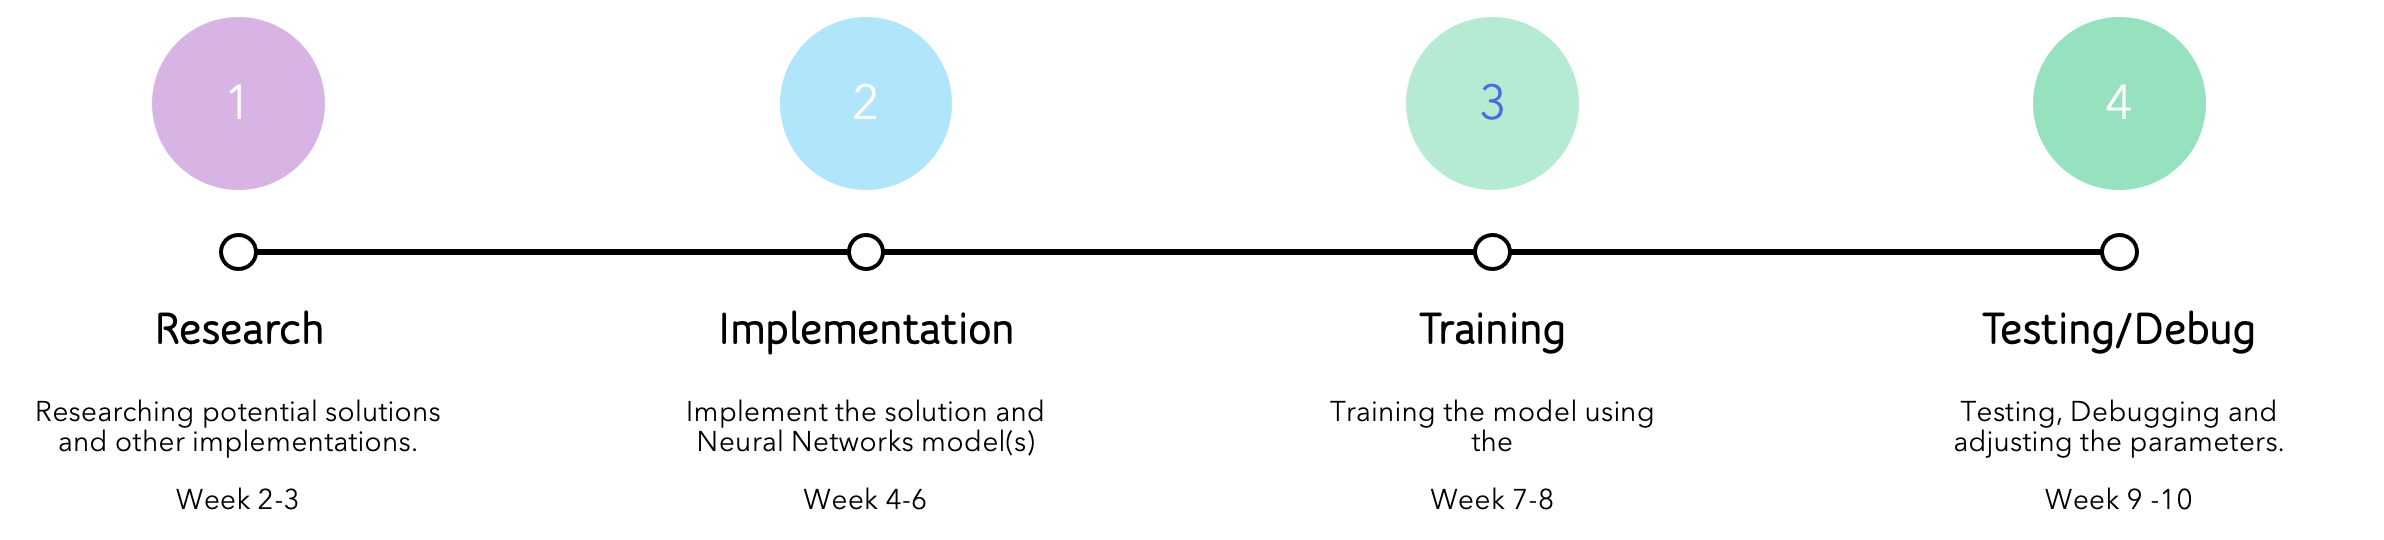
\includegraphics[width=\textwidth]{timeline.png}
\end{figure}

\medskip
\printbibliography %Prints bibliography
\end{document}